\documentclass{article}

\usepackage{xcolor}
\usepackage{titleps}
\usepackage[letterpaper, margin=0.95in]{geometry}
\usepackage{url}
\usepackage{amsmath}
\usepackage{amssymb}
\usepackage{wrapfig}
\usepackage{float}
\usepackage{mathtools}
\usepackage{enumitem}
\usepackage{tabu}
\usepackage{parskip}
\usepackage{natbib}
\usepackage{listings}
\usepackage{tikz}
\usepackage{quiver}
\usepackage{color}

\newcommand{\xb}{\mathbf{x}}
\newcommand{\yb}{\mathbf{y}}
\newcommand{\wb}{\mathbf{w}}
\newcommand{\Xb}{\mathbf{X}}
\newcommand{\Yb}{\mathbf{Y}}
\newcommand{\tr}{^T}
\newcommand{\hb}{\mathbf{h}}
\newcommand{\Hb}{\mathbf{H}}

\DeclareFontShape{OT1}{cmtt}{bx}{n}{<5><6><7><8><9><10><10.95><12><14.4><17.28><20.74><24.88>cmttb10}{}

\definecolor{darkblue}{rgb}{0.2, 0.2, 0.5}
\newcommand{\sol}{~\\\color{darkblue}{\bf Solution:~}}
\usepackage{forest}

\usepackage{hyperref}
\usepackage[color=red]{todonotes}
\usepackage{forest}
\definecolor{light-yellow}{HTML}{FFE5CC}

\usepackage{cleveref}

\newpagestyle{ruled}
{\sethead{Berkeley CS 285}{Deep Reinforcement Learning, Decision Making, and Control}{Fall 2023}\headrule
  \setfoot{}{}{}}
\pagestyle{ruled}

\renewcommand\makeheadrule{\color{black}\rule[-.75\baselineskip]{\linewidth}{0.4pt}}
\renewcommand*\footnoterule{}

\begin{document}
\lstset{basicstyle = \ttfamily,columns=fullflexible,
backgroundcolor = \color{light-yellow}
}

\begin{centering}
    {\Large CS 285 Homework 2: Policy Gradients} \\
    \vspace{.25cm}
    \textbf{Due September 25, 11:59 pm} \\
\end{centering}

\setcounter{section}{2}
\section{Policy Gradients}
\begin{itemize}
\item Create two graphs:
\begin{itemize}
\item In the first graph, compare the learning curves (average return vs. number of environment steps) for the experiments prefixed with \verb|cartpole|. (The small batch experiments.)
\item In the second graph, compare the learning curves for the experiments prefixed with \verb|cartpole_lb|. (The large batch experiments.)
\end{itemize}
\textbf{For all plots in this assignment, the $x$-axis should be number of environment steps, logged as} \verb|Train_EnvstepsSoFar| \textbf{(\textit{not} number of policy gradient iterations).}
\item Answer the following questions briefly: 
\begin{itemize}
\item Which value estimator has better performance without advantage normalization: the trajectory-centric one, or the one using reward-to-go?
\item Did advantage normalization help?
\item Did the batch size make an impact?
\end{itemize}
\item Provide the exact command line configurations (or \texttt{\#@params} settings in Colab) you used to run your experiments, including any parameters changed from their defaults.
\end{itemize}

\begin{sol}
    I provide the learning curve graphs below:
    \begin{figure}[h!]
        \begin{center}
        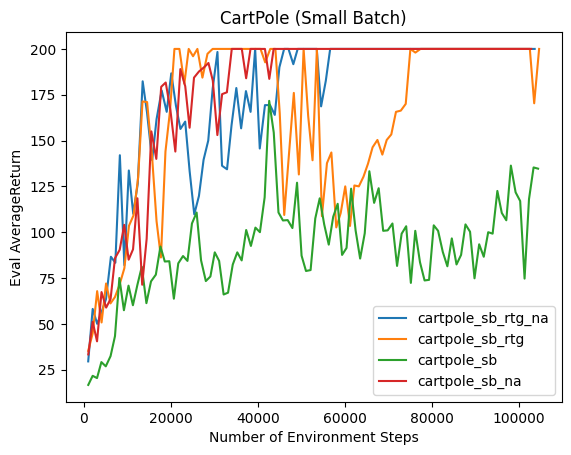
\includegraphics[width=\textwidth/9*4]{q3_cartpole_small_batch.png}
        \hspace*{1cm}
        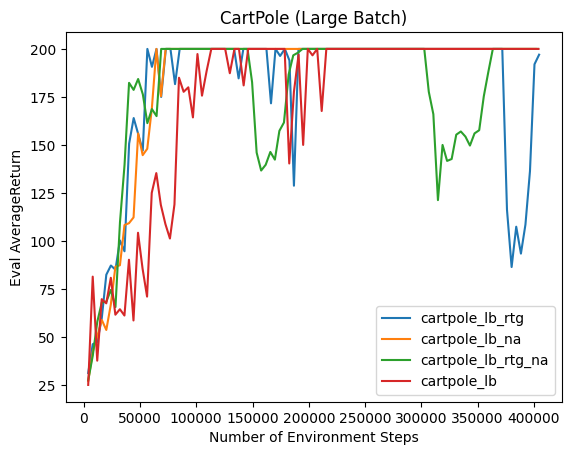
\includegraphics[width=\textwidth/9*4]{q3_cartpole_large_batch.png}
        \end{center}
        \caption{\color{darkblue}The graph on the left displays the learning curves for the small batch runs, and the right displays those of the large batch runs.}
    \end{figure}

    My responses to the questions:
    \begin{itemize}
        \item Without advantage normalization, reward-to-go estimator generally has better performance than the trajectory centric one, as it converges to 200 faster. However, in the large batch experiments, using reward-to-go seems to produce more fluctuations after both reach 200 (e.g. at around environment step 400,000).
        \item Advantage normalization helps significantly with faster convergence and decreased variance upon convergence.
        \item The large batch helped the raw (i.e. no RTG nor NA) policy converge to 200 faster.
        \item The exact command configurations I used are the defaults, provided below:
        \begin{lstlisting}
python cs285/scripts/run_hw2.py --env_name CartPole-v0 -n 100 -b 1000 \
--exp_name cartpole_sb
python cs285/scripts/run_hw2.py --env_name CartPole-v0 -n 100 -b 1000 \
-rtg --exp_name cartpole_sb_rtg
python cs285/scripts/run_hw2.py --env_name CartPole-v0 -n 100 -b 1000 \
-na --exp_name cartpole_sb_na
python cs285/scripts/run_hw2.py --env_name CartPole-v0 -n 100 -b 1000 \
-rtg -na --exp_name cartpole_sb_rtg_na
python cs285/scripts/run_hw2.py --env_name CartPole-v0 -n 100 -b 4000 \
--exp_name cartpole_lb
python cs285/scripts/run_hw2.py --env_name CartPole-v0 -n 100 -b 4000 \
-rtg --exp_name cartpole_lb_rtg
python cs285/scripts/run_hw2.py --env_name CartPole-v0 -n 100 -b 4000 \
-na --exp_name cartpole_lb_na
python cs285/scripts/run_hw2.py --env_name CartPole-v0 -n 100 -b 4000 \
-rtg -na --exp_name cartpole_lb_rtg_na
        \end{lstlisting}
    \end{itemize}
\end{sol}

\newpage\section{Neural Network Baseline}
\begin{itemize}
    \item Plot a learning curve for the baseline loss.
    \item Plot a learning curve for the eval return. You should expect to achieve an average return over 300 for the baselined version.
    \item Run another experiment with a decreased number of baseline gradient steps (\verb|-bgs|) and/or baseline learning rate (\verb|-blr|). How does this affect (a) the baseline learning curve and (b) the performance of the policy?
    \item \textbf{Optional:} Add \verb|-na| back to see how much it improves things. Also, set \verb|video_log_freq 10|, then open TensorBoard and go to the ``Images'' tab to see some videos of your HalfCheetah walking along!
\end{itemize}

\begin{sol}
    I provide the learning curves below:
    \begin{figure}[h!]
        \begin{center}
        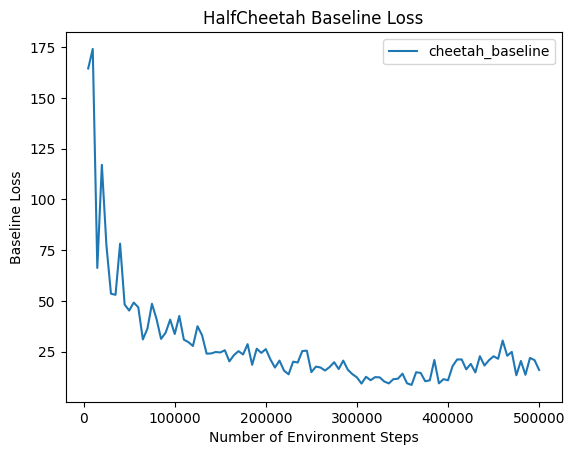
\includegraphics[width=\textwidth/9*4]{q4_cheetah_baseline_loss.png}
        \hspace*{1cm}
        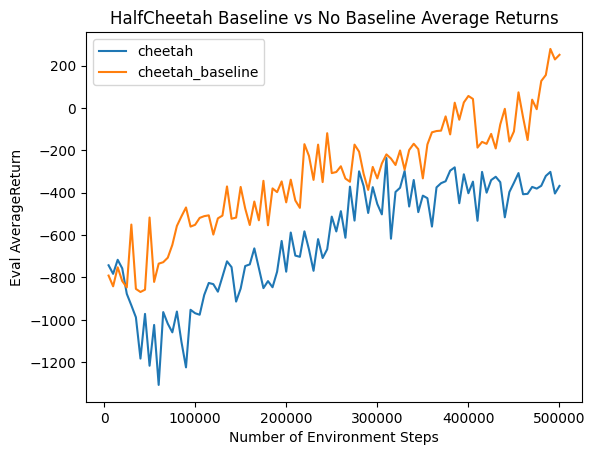
\includegraphics[width=\textwidth/9*4]{q4_cheetah_baseline_avg_returns.png}
        \end{center}
        \caption{\color{darkblue} The graph on the left depicts the learning curve for the baseline loss; the one on the right displays learning curve for the average returns (between using a baseline and not using a baseline). }
    \end{figure}
    \begin{figure}[h!]
        \begin{center}
        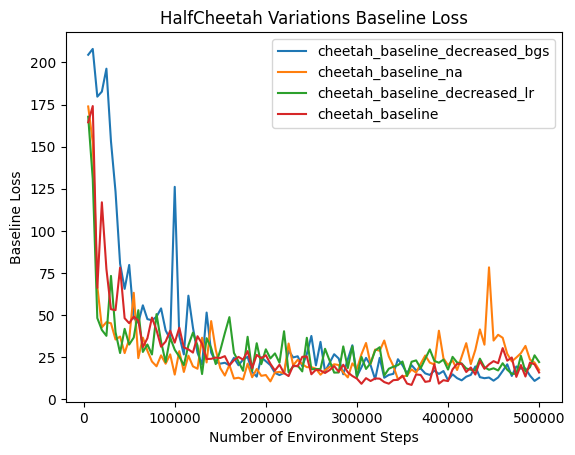
\includegraphics[width=\textwidth/9*4]{q4_cheetah_variations_baseline_loss.png}
        \hspace*{1cm}
        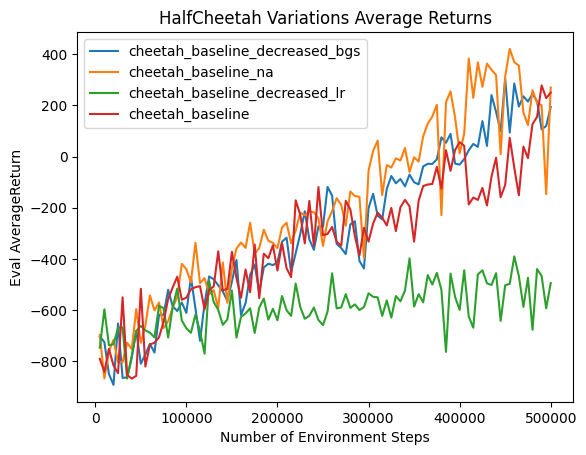
\includegraphics[width=\textwidth/9*4]{q4_cheetah_variations_avg_returns.png}
        \end{center}
        \caption{\color{darkblue} The graph on the left displays the baseline loss curves of the extra experiments, and the right one displays their average return curves.}
    \end{figure}

    For the extra experiments, I tried decreasing the number of baseline gradient steps from 5 to 2, and separately the baseline learning rate from 0.01 to 0.001. I also tried adding advantage normalization to see how it improves things.  
    \begin{itemize}
        \item [(a)] The decreased learning rate helped the baseline loss converge slightly faster, but the decreased number of gradient steps made the convergence slightly slower. 
        \item [(b)] The decreased learning rate worsened the performance of the policy, while the decreased gradient steps didn't significantly impact the performance convergence nor variance.
    \end{itemize}

    The exact command configurations I used are provided below:
    \begin{lstlisting}
# No baseline
python cs285/scripts/run_hw2.py --env_name HalfCheetah-v4 \
-n 100 -b 5000 -rtg --discount 0.95 -lr 0.01 \
--exp_name cheetah

# Baseline
python cs285/scripts/run_hw2.py --env_name HalfCheetah-v4 \
-n 100 -b 5000 -rtg --discount 0.95 -lr 0.01 \
--use_baseline -blr 0.01 -bgs 5 --exp_name cheetah_baseline

# Baseline with advantage normalization
python cs285/scripts/run_hw2.py --env_name HalfCheetah-v4 \
-n 100 -b 5000 -rtg -na --discount 0.95 -lr 0.01 \
--use_baseline -blr 0.01 -bgs 5 --exp_name cheetah_baseline_na

# Baseline with decreased baseline gradient steps
python cs285/scripts/run_hw2.py --env_name HalfCheetah-v4 \
-n 100 -b 5000 -rtg --discount 0.95 -lr 0.01 \
--use_baseline -blr 0.01 -bgs 2 --exp_name cheetah_baseline_decreased_bgs

# Baseline with decreased learning rate
python cs285/scripts/run_hw2.py --env_name HalfCheetah-v4 \
-n 100 -b 5000 -rtg --discount 0.95 -lr 0.001 \
--use_baseline -blr 0.01 -bgs 5 --exp_name cheetah_baseline_decreased_lr
    \end{lstlisting}
\end{sol}

\newpage\section{Generalized Advantage Estimation}
\begin{itemize}
    \item Provide a single plot with the learning curves for the \verb|LunarLander-v2| experiments that you tried. Describe in words how $\lambda$ affected task performance. The run with the best performance should achieve an average score close to 200 (180+).
    \item Consider the parameter $\lambda$. What does $\lambda = 0$ correspond to? What about $\lambda = 1$? Relate this to the task performance in \verb|LunarLander-v2| in one or two sentences.
\end{itemize}

\begin{sol}
    I provide a plot depicting the learning curves for the \texttt{LunarLander-v2} experiments below:
    \begin{figure}[h!]
        \begin{center}
        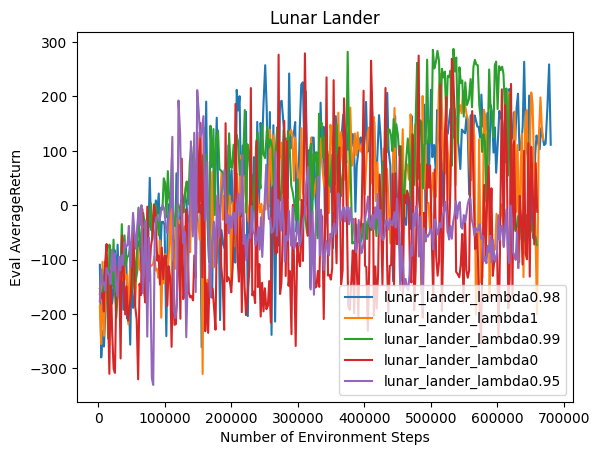
\includegraphics[width=\textwidth*2/3]{q5_lunar_avg_returns.png}
        \end{center}
    \end{figure}

The parameter $\lambda$ represents the balance between prioritizing variance v.s. bias when estimating advantages, in particular through how much we weigh reward accumulation. Thus, $\lambda=0$ corresponds to estimating advantages solely on the rewards at each step, while $\lambda=1$ corresponds to estimating advantages based on accumulated rewards.

In regards to the performance in \texttt{LunarLander-v2}, we see that the highest $\lambda$ values (e.g. 0.99 and 1) perform the best, while the lower values of $\lambda$ perform worse (e.g. 0 and 0.95). In particular, we can see that all the learning curves are relatively similar in the earlier environment steps, but the policies with higher $\lambda$ values begin to perform better later on since they are able to account for accumulating rewards.

The exact command configurations I used are the defaults, provided below:
\begin{lstlisting}
for lambda in 0 0.95 0.98 0.99 1
do
    python cs285/scripts/run_hw2.py \
        --env_name LunarLander-v2 --ep_len 1000 \
        --discount 0.99 -n 300 -l 3 -s 128 -b 2000 -lr 0.001 \
        --use_reward_to_go --use_baseline --gae_lambda $lambda \
        --exp_name lunar_lander_lambda$lambda
done
\end{lstlisting}
\end{sol}

\newpage\section{Hyperparameter Tuning}
\begin{enumerate}
    \item Provide a set of hyperparameters that achieve high return on \verb|InvertedPendulum-v4| in as few environment steps as possible.
    \item Show learning curves for the average returns with your hyperparameters and with the default settings, with environment steps on the $x$-axis. Returns should be averaged over 5 seeds.
\end{enumerate}

\begin{sol}
    The set of hyperparameters that achieve high return on \texttt{InvertedPendulum-v4} is: all defaults except return-to-go is disabled and decrease the batch size from 5000 to 3000. 

    I provide the learning curves below:
    \begin{figure}[h!]
        \begin{center}
        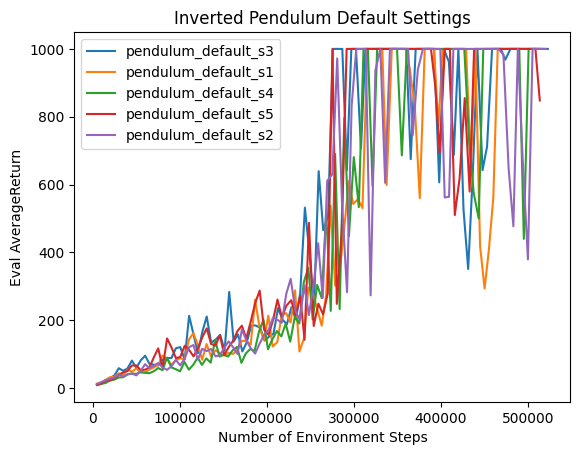
\includegraphics[width=\textwidth/9*4]{q6_ip_default.png}
        \hspace*{1cm}
        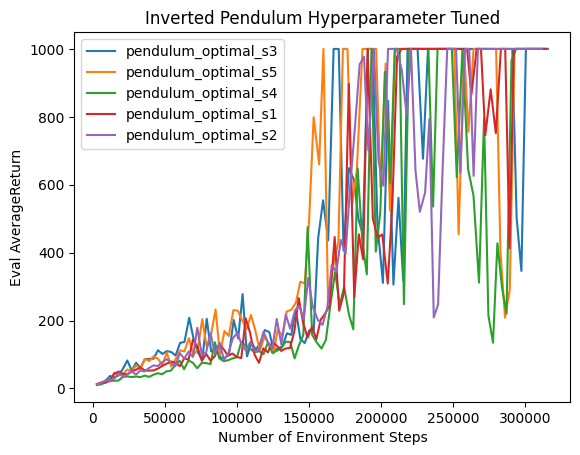
\includegraphics[width=\textwidth/9*4]{q6_ip_optimal.png}
        \end{center}
        \caption{\color{darkblue} The graph on the left displays the learning curves with the default setting, and the one on the right displays the learning curves with my set of hyperparameters. \textbf{We see that my hyperparameter tuning improved the convergence time from around 300,000 environment steps to around around 175,000 environment steps.}}
    \end{figure}

    The exact command configurations I used are provided below:
\begin{lstlisting}
# default settings
for seed in $(seq 1 5); do
    python cs285/scripts/run_hw2.py --env_name InvertedPendulum-v4 -n 100 \
        --exp_name pendulum_default_s$seed \
        -rtg --use_baseline -na \
        --batch_size 5000 \
        --seed $seed
done

# my settings
for seed in $(seq 1 5); do
    python cs285/scripts/run_hw2.py --env_name InvertedPendulum-v4 -n 100 \
    --exp_name pendulum_optimal_s$seed \
    --use_baseline -na \
    --batch_size 3000 \
    --seed $seed
done
\end{lstlisting}

\end{sol}

\newpage\section{(Extra Credit) Humanoid}
\begin{enumerate}
    \item Plot a learning curve for the Humanoid-v4 environment. You should expect to achieve an average return of at least 600 by the end of training. Discuss what changes, if any, you made to complete this problem (for example: optimizations to the original code, hyperparameter changes, algorithmic changes).
\end{enumerate}

\begin{sol}
    I plot the learning curve for the \texttt{Humanoid-v4} environment below:
    \begin{figure}[h!]
        \begin{center}
        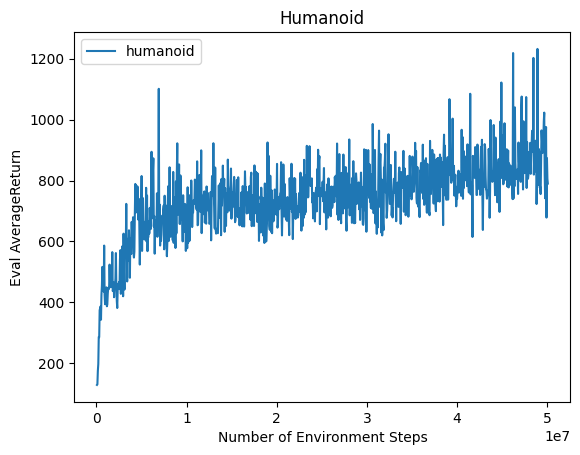
\includegraphics[width=\textwidth*2/3]{q7_humanoid.png}
        \end{center}
        \caption{\color{darkblue} We can see that the policy achieves an average return of far above 600 (i.e. around 900) by the end of training.}
    \end{figure}

    The exact command configurations I used are the defaults, provided below:
\begin{lstlisting}
python cs285/scripts/run_hw2.py \
    --env_name Humanoid-v4 --ep_len 1000 \
    --discount 0.99 -n 1000 -l 3 -s 256 -b 50000 -lr 0.001 \
    --baseline_gradient_steps 50 \
    -na --use_reward_to_go --use_baseline --gae_lambda 0.97 \
    --exp_name humanoid --video_log_freq 5
\end{lstlisting}
\end{sol}

\newpage\section{Analysis}
\label{sec:analysis}
Consider the following infinite-horizon MDP:
% https://q.uiver.app/#q=WzAsMixbMCwwLCJzIl0sWzAsMSwic19GIl0sWzAsMSwiYV8yIl1d
\[\begin{tikzcd}
	s_1 & {s_F}
	\arrow["{a_2}", from=1-1, to=1-2]
    \arrow["{a_1}", loop left, from=1-1, to=1-1]
\end{tikzcd}\]
\newcommand{\Rmax}[0]{R_{\textrm{max}}}
\newcommand{\E}[0]{\mathbb{E}}
\newcommand{\var}[0]{\textrm{Var}}
\crefname{question}{part}{parts}
\Crefname{question}{Part}{Parts}
\newcommand\question[1][]{\item\refstepcounter{subsection}\label[question]{#1}}

At each step, the agent stays in state $s_1$ and receives reward 1 if it takes action $a_1$, and receives reward 0 and terminates the episode otherwise.
Parametrize the policy as stationary (not dependent on time) with a single parameter:
\[\pi_\theta(a_1|s_1) = \theta, \pi_\theta(a_2|s_1) = 1-\theta\]

\begin{enumerate}
\question[sec:analysis1] Applying policy gradients
\begin{enumerate}
    \item Use policy gradients to compute the gradient of the expected return $R(\tau)$ with respect to the parameter $\theta$. \textbf{Do not use discounting.}

    \textbf{Hint}: to compute $\sum_{k=1}^\infty k\alpha^{k-1}$, you can write:
    \[\sum_{k=1}^\infty k\alpha^{k-1} = \sum_{k=1}^\infty \frac{d}{d\alpha}\alpha^k = \frac{d}{d\alpha}\sum_{k=1}^\infty\alpha^k\]

    \begin{sol}
We compute the expected policy gradient as follows: 
\begin{align*}
    \E_{\pi_\theta}\left[\sum_{t \in \mathcal{T}} \nabla_\theta \log \pi_\theta(a_t \mid s_t) R(\tau)\right] &= \sum_{t=1}^{\infty} \theta^t (1 - \theta) \left(\sum_{t'=1}^t \nabla_\theta \log \pi_\theta(a_1) + \nabla_\theta \log \pi_\theta (a_2)\right)t \\
    &= \sum_{t=1}^\infty \theta^t (1 - \theta) \left(\frac{t}{\theta} - \frac{1}{1 - \theta}\right) t \\
    &= \sum_{t=1}^\infty \left(\theta^{t-1} (1 - \theta) t^2 - \theta^t t\right) \\
    &= \sum_{t=1}^\infty \left((\theta^{t-1} - \theta^t) \cdot t(t+1) + (-\theta^{t-1} + \theta^t - \theta^t) \cdot t\right) \\
    &= (1 - \theta) \sum_{t=1}^{\infty} \theta^{t-1} t(t+1) - \sum_{t=1}^{\infty} \theta^{t-1} t \\
    &= (1 - \theta) \cdot \frac{\partial^2}{\partial \theta^2} \left(\frac{\theta}{1 - \theta}\right) - \frac{\partial }{\partial \theta} \left( \frac{1}{1 - \theta}\right) \\
    &= (1 - \theta) \cdot \frac{2}{(1 - \theta)^3} - \frac{1}{(1 - \theta)^2} \\
    &= \frac{1}{(1 - \theta)^2}
\end{align*}
    \end{sol}

    \newpage
    
    \item \label{exact_gradient} Compute the expected return of the policy $\E_{\tau \sim \pi_\theta} R(\tau)$ directly. Compute the gradient of this expression with respect to $\theta$ and verify that this matches the policy gradient.

    \begin{sol}
We compute the expected return directly as follows:
\begin{align*}
    \E_{\tau \sim \pi_\theta} [R(\tau)] &= \E_{\tau \sim \pi_\theta}[t] \\
    &= (1 - \theta) \sum_{t=1}^\infty \theta^t t \\
    &= (1 - \theta) \cdot \frac{\theta}{(1 - \theta)^2} \\
    &= \frac{\theta}{1 - \theta}
\end{align*}
We then compute the gradient of this expression as follows:
\[\frac{\partial}{\partial \theta} \left(\frac{\theta}{1 - \theta}\right) = \frac{1}{(1 - \theta)^2},\]
and confirm that it matches the policy gradient computed in part (a).
    
    \end{sol}

\end{enumerate}
\newpage
\question[sec:analysis2] Compute the variance of the policy gradient in closed form and describe the properties of the variance with respect to $\theta$. For what value(s) of $\theta$ is variance minimal? Maximal? (Once you have an exact expression for the variance you can eyeball the min/max).

\textbf{Hint:}  Once you have it expressed as a sum of terms $P(\theta)/Q(\theta)$ where $P$ and $Q$ are polynomials, you can use a symbolic computing program (Mathematica, SymPy, etc) to simplify to a single rational expression.

\begin{sol}
    We compute the variance of the policy gradient as follows:
\begin{align*}
    &\text{Var}_{\pi_\theta} \left(\sum_{t \in \mathcal{T}} \nabla_\theta \log \pi_\theta(a_t \mid s_t) R(\tau)\right) \\
    &= \E_{\pi_\theta} \left[\left(\sum_{t \in \mathcal{T}} \nabla_\theta \log \pi_\theta(a_t \mid s_t) R(\tau)\right)^2\right] - \E_{\pi_\theta}\left[\sum_{t \in \mathcal{T}} \nabla_\theta \log \pi_\theta(a_t \mid s_t) R(\tau)\right]^2\\
    &= \sum_{t=1}^\infty \theta^t (1 - \theta) \left(\sum_{t' = 1}^t \nabla_\theta \log \pi_\theta(a_1) + \nabla_\theta \log \pi_\theta (a_2)\right)^2 t^2 - \left(\frac{1}{(1 - \theta)^2}\right)^2\\
    &= \sum_{t=1}^\infty \theta^t (1 - \theta) \left(\frac{t}{\theta} - \frac{1}{1 - \theta}\right)^2 t^2  - \frac{1}{(1 - \theta)^4} \\
    &= \sum_{t=1}^\infty \theta^t (1 - \theta) \left(\frac{t^4}{\theta^2} - \frac{2t^3}{\theta (1 - \theta)} + \frac{t^2}{(1 - \theta)^2}\right)  - \frac{1}{(1 - \theta)^4} \\
    &= \frac{4\theta + 9 + \frac{1}{\theta}}{(1 - \theta)^4} - \frac{1}{(1 - \theta)^4} \\
    &= \frac{4\theta + 8 + \frac{1}{\theta}}{(1 - \theta)^4}
\end{align*}
where between lines 4 and 5, we used a symbolic computing program (Wolfram Alpha) to compute the closed form for the left summation.
\end{sol}

\newpage
\question[sec:analysis3] Apply return-to-go as an advantage estimator.
\begin{enumerate}
    \item Write the modified policy gradient and confirm that it is unbiased.

    \begin{sol}
        We compute the expected modified policy gradient as follows, where $T$ is the number of steps taken at $a_1$ before terminating at $a_2$.
        \begin{align*}
            \E_{\pi_\theta}\left[\sum_{t \in \mathcal{T}} \nabla_\theta \log \pi_\theta(a_t \mid s_t) (T - t)\right] &= \sum_{T=1}^\infty \theta^T (1 - \theta) \sum_{t=1}^T \nabla_\theta \log \pi_\theta(a_t \mid s_t) (T - t) \\
            &= \sum_{T=1}^\infty \theta^T(1 - \theta) \cdot \frac{T(T+1)}{2 \theta} \\
            &= \frac{1 - \theta}{2 \theta} \sum_{T=1}^\infty \theta^T T(T+1) \\
            &= \frac{1}{(1 - \theta)^2}
        \end{align*}
        where we used a symbolic computing program to simplify the last step. Thus, we confirm that this modified policy gradient is unbiased.
    \end{sol}

    \item Compute the variance of the return-to-go policy gradient and plot it on $[0, 1]$ alongside the variance of the original estimator.

    \begin{sol}
        We compute the variance of the expected return-to-go policy gradient below:
    \begin{align*}
&\text{Var}_{\pi_\theta}\left(\sum_{t \in \mathcal{T}} \nabla_\theta \log \pi_\theta(a_t \mid s_t) (T - t)\right) \\
&= \E_{\pi_\theta} \left[\left(\sum_{t \in \mathcal{T}} \nabla_\theta \log \pi_\theta(a_t \mid s_t) (T - t)\right)^2\right] - \E_{\pi_\theta} \left[\sum_{t \in \mathcal{T}} \nabla_\theta \log \pi_\theta(a_t \mid s_t) (T - t)\right]^2 \\
&= \sum_{T=1}^\infty \theta^T (1 - \theta) \left(\frac{T (T+1)}{2\theta}\right)^2  - \left(\frac{1}{(1 - \theta)^2}\right)^2\\
&= \frac{1 - \theta}{4\theta^2} \sum_{T=1}^\infty \theta^T T^2(T+1)^2 - \frac{1}{(1 - \theta)^4} \\
&= \frac{\theta + 4 + \frac{1}{\theta}}{(1 - \theta)^4} - \frac{1}{(1 - \theta)^4} \\
&= \frac{\theta + 3 + \frac{1}{\theta}}{(1 - \theta)^4}
    \end{align*}
    Now, we plot this on [0.05, 0.95] (not [0, 1] so that we can compare better) along with the variance of the original estimator below:
    \begin{figure}[h!]
        \begin{center}
        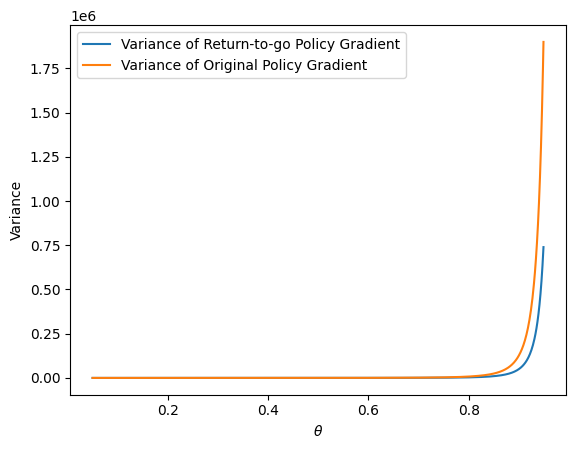
\includegraphics[width=\textwidth*2/3]{q8.3b.png}
        \end{center}
        \caption{\color{darkblue} We see that the return-to-go policy controls the variance better.}
    \end{figure}

    \end{sol}

\end{enumerate}

\newpage

\question[sec:analysis4] Consider a finite-horizon $H$-step MDP with sparse reward:
% https://q.uiver.app/#q=WzAsNixbMCwwLCJzXzEiXSxbMSwwLCJzXzIiXSxbMiwwLCJzXzMiXSxbMiwxLCJzX0YiXSxbMywwLCJcXGRvdHMiXSxbNCwwLCJzX0giXSxbMCwxLCJhXzEiXSxbMSwyLCJhXzEiXSxbMCwzLCJhXzIiLDJdLFsyLDQsImFfMSJdLFs0LDVdLFsxLDMsImFfMiJdLFsyLDMsImFfMiIsMV0sWzQsMywiYV8yIiwxXV0=
\[\begin{tikzcd}
	{s_1} & {s_2} & {s_3} & \dots & {s_H} \\
	&& {s_F}
	\arrow["{a_1}", from=1-1, to=1-2]
	\arrow["{a_1}", from=1-2, to=1-3]
	\arrow["{a_2}"', from=1-1, to=2-3]
	\arrow["{a_1}", from=1-3, to=1-4]
	\arrow[from=1-4, to=1-5]
	\arrow["{a_2}", from=1-2, to=2-3]
	\arrow["{a_2}"{description}, from=1-3, to=2-3]
	\arrow["{a_2}"{description}, from=1-4, to=2-3]
\end{tikzcd}\]

The agent receives reward $\Rmax$ if it arrives at $s_H$ and reward $0$ if it arrives at $s_F$ (a terminal state). In other words, the return for a trajectory $\tau$ is given by:
\[R(\tau) = \begin{cases}1 & \tau \textrm{ ends at } s_H \\ 0 & \tau \textrm{ ends at } s_F \end{cases}\]
Using the same policy parametrization as above, consider off-policy policy gradients via importance sampling. Assume we want to compute policy gradients for a policy $\pi_\theta$ with samples drawn from $\pi_{\theta'}$.
\begin{enumerate}
    \item Write the policy gradient with importance sampling.

    \begin{sol}
        We compute the expected policy gradient with importance sampling below:
        \[\E_{\pi_\theta}\left[\sum_{t \in \mathcal{T}} \nabla_\theta \log \pi_\theta(a_t \mid s_t) R(\tau)\right] = \E_{\pi_{\theta'}}\left[\left(\frac{\theta}{\theta'}\right)^{H} \frac{HR(\tau)}{\theta}\right] = \theta^{H - 1}H\]
    \end{sol}

    \newpage
    \item Compute its variance.
    
    \begin{sol}
        We compute the variance of the policy gradient with importance sampling below:
        \begin{align*}
            &\text{Var}_{\pi_\theta}\left(\sum_{t \in \mathcal{T}} \nabla_\theta \log \pi_\theta(a_t \mid s_t) R(\tau)\right) \\
            &= \E_{\pi_\theta} \left[\left(\sum_{t \in \mathcal{T}} \nabla_\theta \log \pi_\theta(a_t \mid s_t) R(\tau)\right)^2\right] - \E_{\pi_\theta}\left[\sum_{t \in \mathcal{T}} \nabla_\theta \log \pi_\theta(a_t \mid s_t) R(\tau)\right]^2 \\
            &= \E_{\pi_{\theta'}}\left[\left(\frac{\theta}{\theta'}\right)^{2H} \frac{H^2 R(\tau)^2}{\theta^2}\right] - \E_{\pi_{\theta'}}\left[\left(\frac{\theta}{\theta'}\right)^{H} \frac{HR(\tau)}{\theta}\right]^2 \\
            &= \left(\frac{\theta}{\theta'}\right)^{H} \theta^{H - 2} H^2 - \left(\theta^{ H - 1}H\right)^2 \\
            &= \left(\frac{1}{\theta'^H} - 1\right) \cdot \theta^{2H - 2}H^2
        \end{align*}
    \end{sol}

\end{enumerate}

\end{enumerate}

\newpage\section{Survey}
\label{sec:survey}
Please estimate, in minutes, for each problem, how much time you spent (a) writing code and (b) waiting for the results. This will help us calibrate the difficulty for future homeworks. 
\begin{itemize}
    \item \textbf{Policy Gradients:} 3, 0
    \item \textbf{Neural Network Baseline:} 1, 2
    \item \textbf{Generalized Advantage Estimation:} 1, 2
    \item \textbf{Hyperparameters and Sample Efficiency:} 1, 26
    \item \textbf{Humanoid:} 0, 18
    \item \textbf{Analysis -- applying policy gradients:} 2, 0
    \item \textbf{Analysis -- PG variance:} 2, 0
    \item \textbf{Analysis -- return-to-go:} 2, 0
    \item \textbf{Analysis -- importance sampling:} 2, 0
\end{itemize}

\end{document}
